\documentclass[letterpaper,10pt]{extarticle}

%Packages Necessary
\usepackage{tikz}
\usepackage{extsizes}
\usepackage[defaultsans]{droidsans}
\renewcommand*\familydefault{\sfdefault} %% Only if the base font of the document is to be this font style
\usepackage[T1]{fontenc}


\usepackage{pgffor, ifthen}
\newcommand{\notes}[3][\empty]{%
    \noindent Notes\vspace{10pt}\\
    \foreach \n in {1,...,#2}{%
        \ifthenelse{\equal{#1}{\empty}}
            {\rule{#3}{0.5pt}\\}
            {\rule{#3}{0.5pt}\vspace{#1}\\}
        }
}

\pagestyle{empty}

\topmargin       0in
\oddsidemargin   0in
\evensidemargin  0in
\headheight      0in
\headsep         0in
\topskip         0in
\textheight      9in
\textwidth       6.5in

\date{11/14/19}

\begin{document}
 \begin{center}
   \huge\textbf{Forge}\par
 \end{center}
 
 \tikz \draw[rounded corners] (0, 0) rectangle (\textwidth, 8) {};
 
 \bigskip
 
 \textit{\parbox{\textwidth}{The Forge takes in the raw elements of industry and turns them into the trappings of higher civilization. Particularly those trappings that kill things.}}

 \begin{center}
   \large\textbf{Costs}\par
 \end{center}
 
\begin{center}
\huge
\begin{tabular}[c]{|p{8cm}|p{8cm}|}
\hline
\begin{center} Wood: \\[5pt] 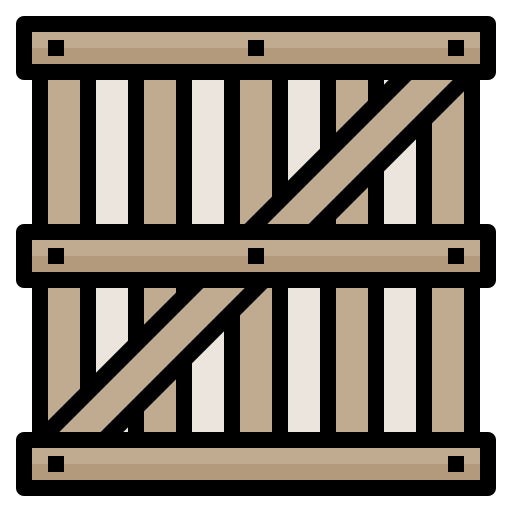
\includegraphics[width=24pt,height=24pt]{../pic/Wood.png}\end{center} & \begin{center} Steel: \\[5pt] 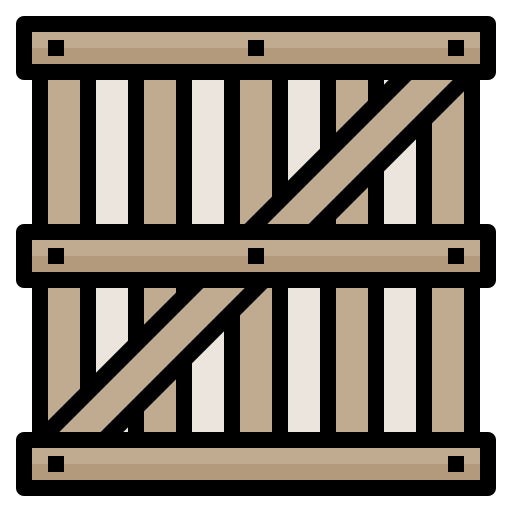
\includegraphics[width=24pt,height=24pt]{../pic/Steel.png}\hspace{12pt}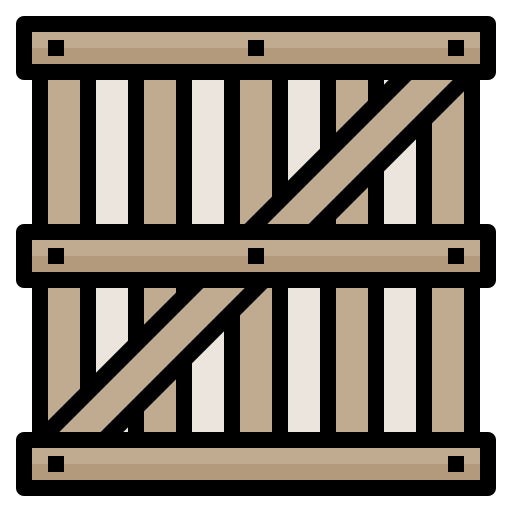
\includegraphics[width=24pt,height=24pt]{../pic/Steel.png}\end{center}\\
\hline
\begin{center} Stone: \\[5pt] 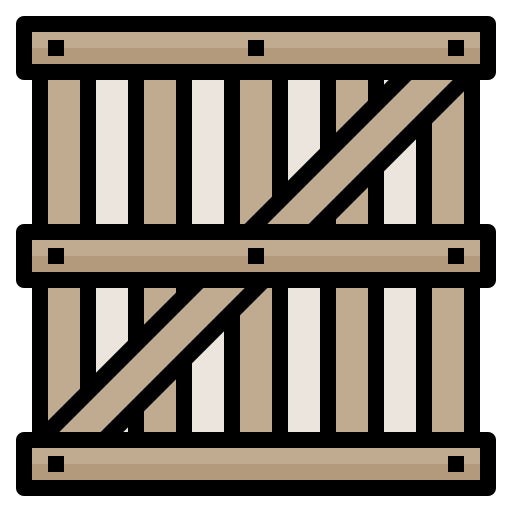
\includegraphics[width=24pt,height=24pt]{../pic/Stone.png}\end{center} & \begin{center} Aetherium: \\[5pt] \end{center}\\
\hline
\begin{center} Phlogiston: \\[5pt] \end{center} & \begin{center} Schicksalcite: \\[5pt] \end{center}\\
\hline
\end{tabular}
\end{center}




 
\newpage
 \begin{center}
   \large\textbf{Requirements}\par
 \end{center}
The Forge must be built In Supply.
\begin{center}
   \large\textbf{Effects}\par
 \end{center}
 
The Forge can be activated with the Craft Gear Development Action by the Guilds Player. Once activated, any amount of Gear Cards can be created as long as the resource costs are paid. The Forge can craft any Gear Cards from the Forge Gear Deck. There are also Gear Decks that require activating the Forge as an additional requirement. When a Gear Card is made, it is immediately added to the Guilds Player's Inventory. From there the Guilds Player may give it to anyone they choose.

\begin{itemize}
\item{Crafts Gear from the Forge Deck}
\item{Required to Craft Gear from the Technoforge, the Cryptoworkshop, and the Skycarpentry.}
\end{itemize}



 \bigskip
 \bigskip
 \Huge Location: \hspace{2em} \tikz[baseline=-1] \draw (0,-0.75) rectangle (4,1.25);
\end{document}
